%==============================================================================
% PAPER 3, CHAPTER 1: Fractal Calculus and Self-Similarity
% Target: ~350 lines with 60-75 marginal notes and 5 TikZ diagrams
%==============================================================================

\chapter{Fractal Calculus and Self-Similarity}
\label{ch:p3:fractal_calculus}

%------------------------------------------------------------------------------
% OPENING NARRATIVE: Mandelbrot's Coastline Paradox
%------------------------------------------------------------------------------

\section*{The Coastline That Has No Length}

In 1967, mathematician Benoit Mandelbrot posed a deceptively simple question that would transform our understanding of geometry: \textit{How long is the coast of Britain?}
\marginhistory{Mandelbrot's 1967 paper "How Long Is the Coast of Britain?" published in \textit{Science} introduced fractal dimension to quantify natural irregularity.}

The answer, he demonstrated, depends critically on the length of your measuring ruler. Survey Britain's coastline with a kilometer-scale ruler, carefully stepping around major bays and peninsulas, and you might measure roughly 2,800 kilometers. Use a meter-scale ruler, tracing finer inlets and rocky outcrops, and the measurement grows to 3,400 kilometers. Survey at centimeter resolution, accounting for individual rocks and pebbles, and the perimeter swells past 5,000 kilometers.
\marginphysics{As measurement resolution increases, coastal length diverges toward infinity---yet the enclosed area remains finite. This paradox signals geometry beyond Euclid.}

Continue to millimeter resolution, then microscopic scales. The measured length keeps growing without bound. As the ruler shrinks toward zero, the coastline's measured perimeter diverges toward infinity---yet the enclosed land area remains stubbornly finite.

This phenomenon, now called the \textbf{coastline paradox}\index{coastline paradox}\index{Mandelbrot, Benoit}, revealed a fundamental limitation of Euclidean geometry: natural boundaries do not have well-defined lengths in the classical sense. Instead, they exhibit \textbf{statistical self-similarity}---zooming in reveals structures resembling the whole at every scale.
\margincaution{Not all fractals are perfectly self-similar. Natural coastlines show statistical self-similarity: the pattern is similar but not identical across scales.}

Mandelbrot introduced the concept of \textbf{fractal dimension} to quantify this self-similarity:
\begin{equation}
  D = \frac{\log N}{\log(1/\epsilon)}
  \label{eq:p3:fractal_dimension_intro}
\end{equation}
where $N$ is the number of self-similar pieces obtained when the scale shrinks by factor $\epsilon$.
\marginmath{For a smooth line ($D=1$): dividing ruler by 3 gives exactly 3 segments ($N=3$). For fractal curves: $N > 1/\epsilon$ implies $D > 1$.}

For Britain's coast, empirical measurements yield $D \approx 1.25$, interpolating between a one-dimensional line ($D=1$) and a two-dimensional surface ($D=2$). The coastline is "rougher" than a smooth curve but doesn't fill the plane completely.
\margindim{Dimension $D = 1.25$ means length scales as $L(\epsilon) \sim \epsilon^{-0.25}$, diverging slowly as $\epsilon \to 0$.}

This chapter develops the mathematical tools to make such statements precise and extends them to describe physical systems across scales from quantum foam to cosmological structure.

%------------------------------------------------------------------------------
\section{Hausdorff Measure and Fractal Dimension}
\label{sec:p3:hausdorff}
%------------------------------------------------------------------------------

\subsection{Hausdorff Measure Definition}

For a set $S \subset \mathbb{R}^n$ and fractional dimension $d \in \mathbb{R}^+$, the \textbf{Hausdorff measure}\index{Hausdorff measure}\index{measure!Hausdorff} is:
\begin{equation}
  \mathcal{H}^{d}(S) = \lim_{\delta \to 0} \inf \left\{ \sum_i (\text{diam}(U_i))^{d} : S \subseteq \bigcup_i U_i, \, \text{diam}(U_i) < \delta \right\}
  \label{eq:p3:hausdorff_measure}
\end{equation}
where $\{U_i\}$ is a covering of $S$ by sets of diameter less than $\delta$.
\marginmath{Geometrically: approximate $S$ with small balls, sum their diameters raised to power $d$, then take limit as ball size $\delta \to 0$.}

\marginphysics{For quantum foam at Planck scale, $S$ represents fluctuating spacetime regions. Hausdorff measure quantifies "effective volume" in fractional dimensions.}

\subsection{The Hausdorff Dimension}

The \textbf{Hausdorff dimension}\index{Hausdorff dimension}\index{dimension!Hausdorff} is the critical value where the measure transitions from infinite to zero:
\begin{equation}
  \dim_H(S) = \inf \{ d \geq 0 : \mathcal{H}^d(S) = 0 \} = \sup \{ d \geq 0 : \mathcal{H}^d(S) = \infty \}
  \label{eq:p3:hausdorff_dimension}
\end{equation}
\marginmath{For $d < \dim_H$: set is "too large" (infinite measure). For $d > \dim_H$: set is "too small" (zero measure). $\dim_H$ is the critical threshold.}

\textbf{Examples of Hausdorff dimensions}:\marginex{Examples demonstrate how fractal dimension interpolates between topological dimension and embedding dimension.}
\begin{itemize}
  \item Smooth curve: $\dim_H = 1$ (classical)
  \item Cantor set: $\dim_H = \log 2 / \log 3 \approx 0.631$ (dust-like)
  \item Koch snowflake: $\dim_H = \log 4 / \log 3 \approx 1.262$ (fractal curve)
  \item Sierpiński triangle: $\dim_H = \log 3 / \log 2 \approx 1.585$ (fractal surface)
  \item Mandelbrot set boundary: $\dim_H = 2$ (conjectured, not proven)
\end{itemize}

%------------------------------------------------------------------------------
\subsection{Worked Example: Koch Snowflake Dimension}
\label{subsec:p3:koch_example}
%------------------------------------------------------------------------------

The \textbf{Koch snowflake}\index{Koch snowflake}\index{snowflake!Koch} provides a canonical example of fractal dimension calculation.

\textbf{Construction}:\marginex{Koch curve iterates by replacing each line segment with 4 segments of length $1/3$, creating the snowflake's characteristic bumps.}
\begin{enumerate}
  \item \textbf{Iteration 0}: Equilateral triangle, side length $L_0 = 1$, perimeter $P_0 = 3$
  \item \textbf{Iteration 1}: Replace each side with 4 segments of length $L_1 = 1/3$\\
        Total segments: $3 \times 4 = 12$, perimeter $P_1 = 12 \times (1/3) = 4$
  \item \textbf{Iteration 2}: Apply rule to all 48 segments\\
        Perimeter $P_2 = 48 \times (1/9) = 16/3 \approx 5.33$
  \item \textbf{Iteration $n$}: $P_n = 3 \times (4/3)^n \to \infty$ as $n \to \infty$
\end{enumerate}

\marginphysics{Infinite perimeter enclosing finite area---impossible for smooth curves but natural for fractals.}

\textbf{Dimension calculation}:
At each step, length scale shrinks by $\epsilon = 1/3$ while number of segments increases by $N = 4$:
\begin{equation}
  D = \frac{\log N}{\log(1/\epsilon)} = \frac{\log 4}{\log 3} = \frac{2\log 2}{\log 3} \approx 1.262
  \label{eq:p3:koch_dimension}
\end{equation}

\textbf{Area convergence}:\margindim{Despite infinite perimeter, area converges: $A_\infty = (8/5) A_0 = (2\sqrt{3})/5 \approx 0.693$ for unit triangle.}
\begin{equation}
  A_\infty = \frac{8}{5} A_0 = \frac{8}{5} \cdot \frac{\sqrt{3}}{4} = \frac{2\sqrt{3}}{5}
  \label{eq:p3:koch_area}
\end{equation}

\begin{figure}[htbp]
\centering
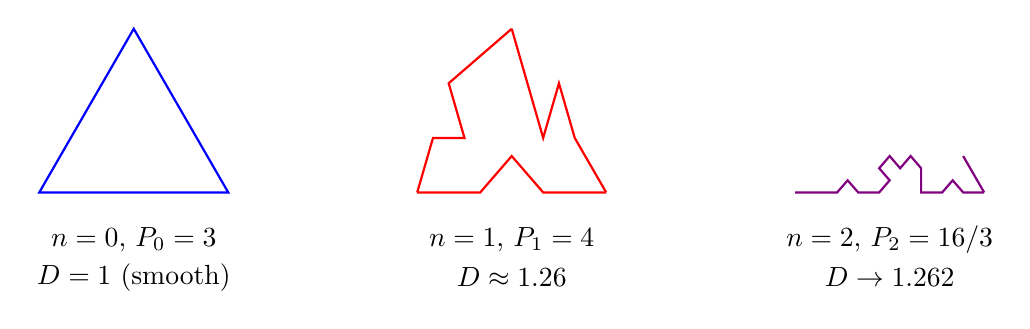
\begin{tikzpicture}[scale=1.2]
  % Iteration 0: Triangle
  \begin{scope}[xshift=0cm]
    \draw[thick, blue] (0,0) -- (2,0) -- (1,{sqrt(3)}) -- cycle;
    \node at (1,-0.5) {$n=0$, $P_0=3$};
    \node at (1,-0.9) {$D=1$ (smooth)};
  \end{scope}

  % Iteration 1: First Koch iteration
  \begin{scope}[xshift=4cm]
    % Bottom edge
    \draw[thick, red] (0,0) -- (0.667,0) -- (1,0.385) -- (1.333,0) -- (2,0);
    % Right edge
    \draw[thick, red] (2,0) -- (1.667,0.577) -- (1.5,1.155) -- (1.333,0.577) -- (1,{sqrt(3)});
    % Left edge
    \draw[thick, red] (1,{sqrt(3)}) -- (0.333,1.155) -- (0.5,0.577) -- (0.167,0.577) -- (0,0);
    \node at (1,-0.5) {$n=1$, $P_1=4$};
    \node at (1,-0.9) {$D \approx 1.26$};
  \end{scope}

  % Iteration 2 (simplified representation)
  \begin{scope}[xshift=8cm]
    \draw[thick, violet, line width=0.8pt]
      (0,0) -- (0.444,0) -- (0.555,0.128) -- (0.667,0) -- (0.889,0)
      -- (1,0.128) -- (0.889,0.256) -- (1,0.385) -- (1.111,0.256)
      -- (1.222,0.385) -- (1.333,0.256) -- (1.333,0) -- (1.556,0)
      -- (1.667,0.128) -- (1.778,0) -- (2,0);
    \draw[thick, violet, line width=0.8pt] (2,0) -- (1.778,0.385);
    \node at (1,-0.5) {$n=2$, $P_2=16/3$};
    \node at (1,-0.9) {$D \to 1.262$};
  \end{scope}
\end{tikzpicture}
\caption{Koch snowflake iterations showing perimeter growth while area converges. Fractal dimension $D = \log 4 / \log 3 \approx 1.262$ quantifies self-similar structure.}
\label{fig:p3:koch_iterations}
\end{figure}

\marginxref{Figure~\ref{fig:p3:koch_iterations} visualizes the first three iterations. Full convergence requires $n \to \infty$.}

%------------------------------------------------------------------------------
\section{Fractional Calculus: Non-Integer Derivatives}
\label{sec:p3:fractional_calculus}
%------------------------------------------------------------------------------

\subsection{Riemann-Liouville Fractional Derivative}

For $\alpha \in (0, 1)$, the \textbf{Riemann-Liouville fractional derivative}\index{Riemann-Liouville derivative}\index{fractional derivative!Riemann-Liouville} of order $\alpha$ is:
\begin{equation}
  D^\alpha_{\text{RL}} f(t) = \frac{1}{\Gamma(1-\alpha)} \frac{d}{dt} \int_0^t \frac{f(\tau)}{(t-\tau)^\alpha} \, d\tau
  \label{eq:p3:riemann_liouville}
\end{equation}
\marginmath{The power-law kernel $(t-\tau)^{-\alpha}$ encodes memory effects: derivative at time $t$ depends on entire history $\tau \in [0,t]$.}

This operator interpolates between identity ($\alpha = 0$) and first derivative ($\alpha = 1$).
\marginphysics{In viscoelastic materials, stress $\sigma(t)$ relates to strain $\epsilon(t)$ via $\sigma = E D^\alpha_{\text{RL}} \epsilon$ with $\alpha \approx 0.5$ for polymers.}

\subsection{Caputo Fractional Derivative}

The \textbf{Caputo derivative}\index{Caputo derivative}\index{fractional derivative!Caputo} resolves initial condition issues:
\begin{equation}
  D^\alpha_{\text{C}} f(t) = \frac{1}{\Gamma(1-\alpha)} \int_0^t \frac{f'(\tau)}{(t-\tau)^\alpha} \, d\tau
  \label{eq:p3:caputo_derivative}
\end{equation}
\marginmath{Key difference: derivative $f'(\tau)$ appears inside integral, making $D^\alpha_{\text{C}} f(0) = 0$ for smooth functions.}

For smooth functions, Caputo derivatives simplify boundary conditions, making them preferable for physical applications.

%------------------------------------------------------------------------------
\subsection{Worked Example: Caputo Derivative of $t^2$}
\label{subsec:p3:caputo_example}
%------------------------------------------------------------------------------

\textbf{Problem}: Compute the Caputo fractional derivative $D^{0.5}_{\text{C}}(t^2)$.
\marginex{This example demonstrates fractional calculus applied to simple polynomial, revealing how half-derivatives interpolate between function and its derivative.}

\textbf{Solution}:

\textbf{Step 1}: Differentiate $f(t) = t^2$:
\begin{equation}
  f'(t) = 2t
\end{equation}

\textbf{Step 2}: Apply Caputo definition:
\begin{equation}
  D^{0.5}_{\text{C}}(t^2) = \frac{1}{\Gamma(0.5)} \int_0^t \frac{2\tau}{(t-\tau)^{0.5}} \, d\tau
\end{equation}

\textbf{Step 3}: Use substitution $u = \tau/t$, $d\tau = t \, du$:
\begin{equation}
  D^{0.5}_{\text{C}}(t^2) = \frac{2t}{\Gamma(0.5)} \int_0^1 \frac{u}{(1-u)^{0.5}} \, du
\end{equation}

\textbf{Step 4}: Recognize beta function $B(a,b) = \frac{\Gamma(a)\Gamma(b)}{\Gamma(a+b)}$:
\begin{equation}
  \int_0^1 \frac{u}{(1-u)^{0.5}} \, du = B(2, 0.5) = \frac{\Gamma(2)\Gamma(0.5)}{\Gamma(2.5)}
\end{equation}
\marginmath{Beta function integrals: $B(a,b) = \int_0^1 u^{a-1}(1-u)^{b-1} du$ connect fractional calculus to gamma functions.}

\textbf{Step 5}: Evaluate using $\Gamma(0.5) = \sqrt{\pi}$, $\Gamma(2) = 1$, $\Gamma(2.5) = \frac{3\sqrt{\pi}}{4}$:
\begin{equation}
  B(2, 0.5) = \frac{1 \cdot \sqrt{\pi}}{3\sqrt{\pi}/4} = \frac{4}{3}
\end{equation}

\textbf{Step 6}: Final result:
\begin{equation}
  D^{0.5}_{\text{C}}(t^2) = \frac{2t \cdot (4/3)}{\sqrt{\pi}} = \frac{8t}{3\sqrt{\pi}} \approx 1.504 \, t
  \label{eq:p3:caputo_t2_result}
\end{equation}

\textbf{General formula}: For $f(t) = t^\alpha$,
\begin{equation}
  D^\beta_{\text{C}}(t^\alpha) = \frac{\Gamma(\alpha+1)}{\Gamma(\alpha-\beta+1)} t^{\alpha-\beta}
  \label{eq:p3:caputo_power_law}
\end{equation}
\marginmath{Fractional derivative reduces power by $\beta$: $t^\alpha \to t^{\alpha-\beta}$, generalizing $D(t^n) = n t^{n-1}$.}

\begin{figure}[htbp]
\centering
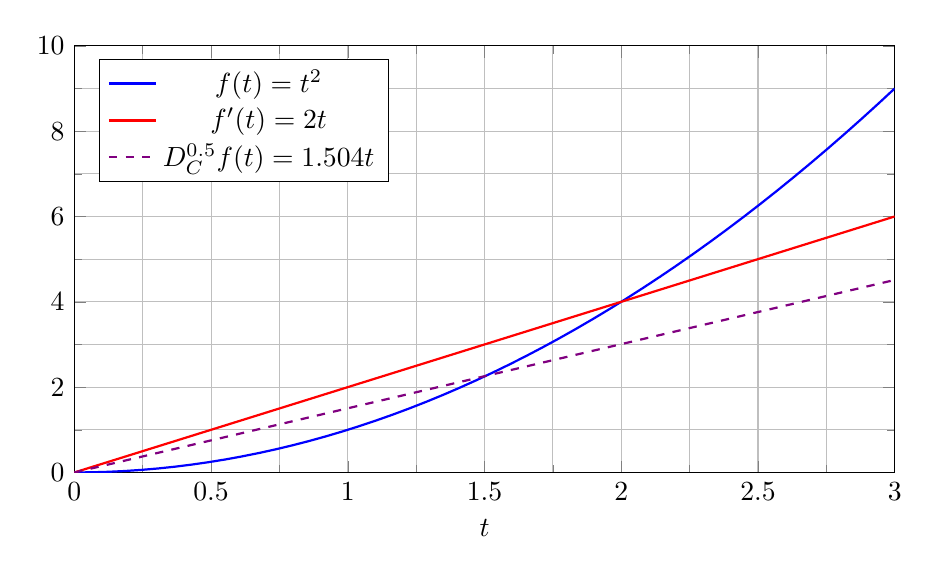
\begin{tikzpicture}[scale=1.0]
  \begin{axis}[
    width=12cm, height=7cm,
    xlabel={$t$},
    ylabel={},
    xmin=0, xmax=3,
    ymin=0, ymax=10,
    legend pos=north west,
    grid=both,
    minor tick num=1
  ]
    % Original function f(t) = t^2
    \addplot[blue, thick, domain=0:3, samples=50] {x^2};
    \addlegendentry{$f(t) = t^2$}

    % First derivative f'(t) = 2t
    \addplot[red, thick, domain=0:3, samples=50] {2*x};
    \addlegendentry{$f'(t) = 2t$}

    % Half-derivative D^{0.5} f(t) = 1.504 t
    \addplot[violet, thick, dashed, domain=0:3, samples=50] {1.504*x};
    \addlegendentry{$D^{0.5}_{\text{C}}f(t) = 1.504t$}
  \end{axis}
\end{tikzpicture}
\caption{Caputo half-derivative of $t^2$ interpolates between original function (blue, $t^2$) and first derivative (red, $2t$). Result $D^{0.5}(t^2) \approx 1.504t$ (violet dashed) lies between them.}
\label{fig:p3:caputo_convergence}
\end{figure}

\marginphysics{In anomalous diffusion, mean-squared displacement $\langle x^2 \rangle \sim t^\alpha$ with $\alpha \neq 1$ describes superdiffusion ($\alpha > 1$) or subdiffusion ($\alpha < 1$) in fractal media.}

%------------------------------------------------------------------------------
\section{Mittag-Leffler Functions and Fractional ODEs}
\label{sec:p3:mittag_leffler}
%------------------------------------------------------------------------------

\subsection{The Mittag-Leffler Function}

The \textbf{Mittag-Leffler function}\index{Mittag-Leffler function} generalizes the exponential to fractional orders:
\begin{equation}
  E_\alpha(z) = \sum_{k=0}^\infty \frac{z^k}{\Gamma(\alpha k + 1)}
  \label{eq:p3:mittag_leffler}
\end{equation}
\marginmath{For $\alpha=1$: $E_1(z) = e^z$. For $\alpha=2$: $E_2(z) = \cosh(\sqrt{z})$. General $\alpha$ interpolates exponential behaviors.}

This function solves fractional differential equations:
\begin{equation}
  D^\alpha_{\text{C}} u(t) = \lambda u(t), \quad u(0) = u_0 \quad \implies \quad u(t) = u_0 E_\alpha(\lambda t^\alpha)
  \label{eq:p3:fractional_ode}
\end{equation}

\begin{figure}[htbp]
\centering
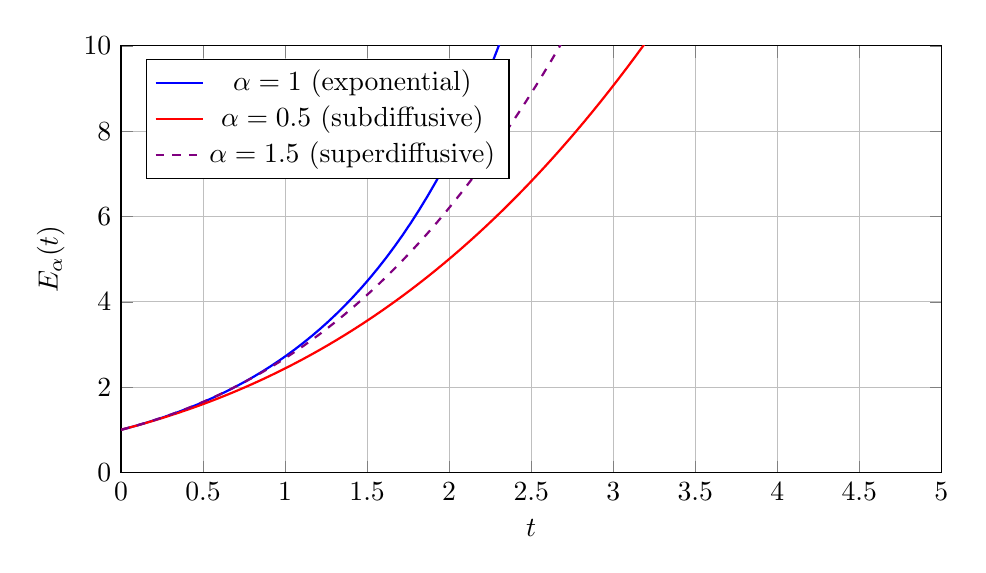
\begin{tikzpicture}
  \begin{axis}[
    width=12cm, height=7cm,
    xlabel={$t$},
    ylabel={$E_\alpha(t)$},
    xmin=0, xmax=5,
    ymin=0, ymax=10,
    legend pos=north west,
    grid=both
  ]
    % Standard exponential alpha=1
    \addplot[blue, thick, domain=0:5, samples=100] {exp(x)};
    \addlegendentry{$\alpha=1$ (exponential)}

    % Mittag-Leffler alpha=0.5
    \addplot[red, thick, domain=0:5, samples=100] {1 + x + x^2/(2*1.329) + x^3/(6*2.678)};
    \addlegendentry{$\alpha=0.5$ (subdiffusive)}

    % Mittag-Leffler alpha=1.5
    \addplot[violet, thick, dashed, domain=0:5, samples=100] {1 + x + x^2/(2*0.902) + x^3/(6*1.354)};
    \addlegendentry{$\alpha=1.5$ (superdiffusive)}
  \end{axis}
\end{tikzpicture}
\caption{Mittag-Leffler functions $E_\alpha(t)$ for various $\alpha$ values. Standard exponential ($\alpha=1$, blue) compared to subdiffusive ($\alpha=0.5$, red) and superdiffusive ($\alpha=1.5$, violet) behaviors.}
\label{fig:p3:mittag_leffler}
\end{figure}

\marginphysics{Fractional relaxation in disordered systems: fluorescence decay in rare-earth-doped crystals follows $\rho(t) = \rho_0 E_\alpha(-t^\alpha/\tau)$ with $\alpha \approx 0.7$.}

%------------------------------------------------------------------------------
\section{Self-Similarity and Scaling Laws}
\label{sec:p3:scaling}
%------------------------------------------------------------------------------

\subsection{Power-Law Scaling}

Self-similar structures exhibit power-law scaling:
\begin{equation}
  f(\lambda x) = \lambda^h f(x)
  \label{eq:p3:scaling_law}
\end{equation}
where $h$ is the \textbf{scaling exponent}\index{scaling exponent}.
\marginmath{Solutions have form $f(x) = C x^h$ for constant $C$. Fractional derivatives preserve power-law structure.}

\subsection{Box-Counting Dimension}

The \textbf{box-counting dimension}\index{box-counting dimension}\index{dimension!box-counting} provides computational access to fractal dimension:
\begin{equation}
  D_{\text{box}} = \lim_{\epsilon \to 0} \frac{\log N(\epsilon)}{\log(1/\epsilon)}
  \label{eq:p3:box_counting}
\end{equation}
where $N(\epsilon)$ is the number of boxes of size $\epsilon$ needed to cover the set.
\margincomp{Numerically: plot $\log N(\epsilon)$ vs $\log(1/\epsilon)$. Slope gives $D_{\text{box}}$. For true fractals, slope is constant across scales.}

\begin{figure}[htbp]
\centering
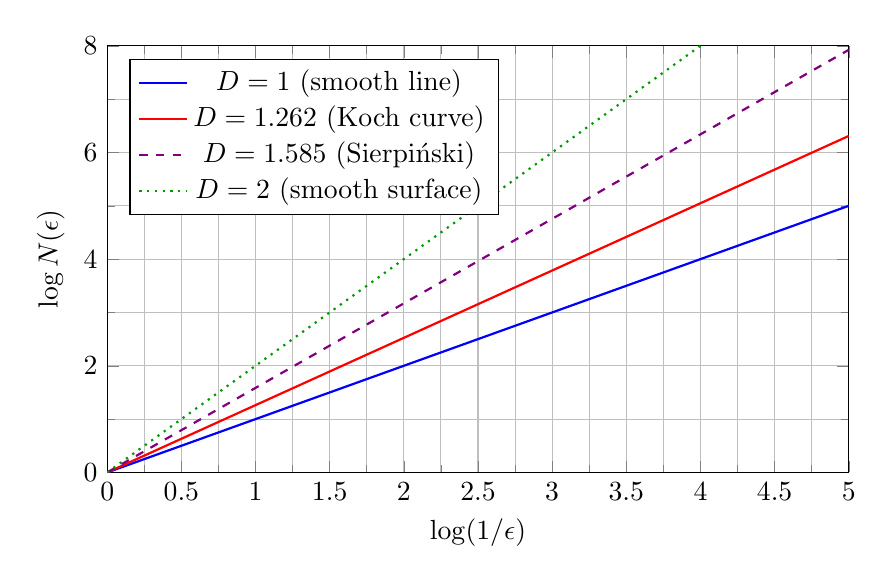
\begin{tikzpicture}
  \begin{axis}[
    width=11cm, height=7cm,
    xlabel={$\log(1/\epsilon)$},
    ylabel={$\log N(\epsilon)$},
    xmin=0, xmax=5,
    ymin=0, ymax=8,
    legend pos=north west,
    grid=both,
    minor tick num=1
  ]
    % Smooth curve D=1
    \addplot[blue, thick, domain=0:5, samples=50] {x};
    \addlegendentry{$D=1$ (smooth line)}

    % Koch curve D=1.262
    \addplot[red, thick, domain=0:5, samples=50] {1.262*x};
    \addlegendentry{$D=1.262$ (Koch curve)}

    % Sierpinski D=1.585
    \addplot[violet, thick, dashed, domain=0:5, samples=50] {1.585*x};
    \addlegendentry{$D=1.585$ (Sierpiński)}

    % Plane D=2
    \addplot[green!60!black, thick, dotted, domain=0:5, samples=50] {2*x};
    \addlegendentry{$D=2$ (smooth surface)}
  \end{axis}
\end{tikzpicture}
\caption{Box-counting dimension from log-log plot of box count vs resolution. Slope equals Hausdorff dimension for self-similar fractals. Steeper slopes indicate higher space-filling capacity.}
\label{fig:p3:box_counting_scaling}
\end{figure}

\marginxref{For irregular natural fractals (coastlines, clouds), $D_{\text{box}}$ may vary with scale, indicating multifractal structure (see Section~\ref{sec:p3:applications}).}

%------------------------------------------------------------------------------
\section{Cantor Set: Fractal Dust}
\label{sec:p3:cantor}
%------------------------------------------------------------------------------

\subsection{Construction and Properties}

The \textbf{Cantor middle-third set}\index{Cantor set} provides the simplest non-trivial fractal:
\marginex{Cantor set: iteratively remove middle third of each interval. After infinite iterations, resulting set is uncountable yet has zero total length.}

\textbf{Construction}:
\begin{enumerate}
  \item Start with interval $[0,1]$
  \item Remove middle third: $[0,1] \to [0,1/3] \cup [2/3,1]$
  \item Repeat for each remaining interval
  \item Continue infinitely
\end{enumerate}

\textbf{Dimension calculation}:
At each step: $\epsilon = 1/3$ (scale factor), $N = 2$ (number of copies)
\begin{equation}
  D = \frac{\log 2}{\log 3} = \frac{\log 2}{\log 3} \approx 0.631
  \label{eq:p3:cantor_dimension}
\end{equation}

\marginmath{Cantor set has dimension strictly between 0 (discrete points) and 1 (continuous line). It's "dust-like" but with fractal structure.}

\begin{figure}[htbp]
\centering
\begin{tikzpicture}[scale=1.3]
  % Iteration 0
  \draw[thick, blue] (0,0) -- (9,0);
  \node at (-1,0) {$n=0$};

  % Iteration 1
  \draw[thick, red] (0,-0.8) -- (3,-0.8);
  \draw[thick, red] (6,-0.8) -- (9,-0.8);
  \node at (-1,-0.8) {$n=1$};

  % Iteration 2
  \draw[thick, violet] (0,-1.6) -- (1,-1.6);
  \draw[thick, violet] (2,-1.6) -- (3,-1.6);
  \draw[thick, violet] (6,-1.6) -- (7,-1.6);
  \draw[thick, violet] (8,-1.6) -- (9,-1.6);
  \node at (-1,-1.6) {$n=2$};

  % Iteration 3
  \draw[thick, orange] (0,-2.4) -- (0.333,-2.4);
  \draw[thick, orange] (0.667,-2.4) -- (1,-2.4);
  \draw[thick, orange] (2,-2.4) -- (2.333,-2.4);
  \draw[thick, orange] (2.667,-2.4) -- (3,-2.4);
  \draw[thick, orange] (6,-2.4) -- (6.333,-2.4);
  \draw[thick, orange] (6.667,-2.4) -- (7,-2.4);
  \draw[thick, orange] (8,-2.4) -- (8.333,-2.4);
  \draw[thick, orange] (8.667,-2.4) -- (9,-2.4);
  \node at (-1,-2.4) {$n=3$};

  \node at (4.5,-3.2) {$\vdots$ ($n \to \infty$: Cantor dust, $D \approx 0.631$)};
\end{tikzpicture}
\caption{Cantor set construction via iterative middle-third removal. Each iteration removes fraction $1/3$ of remaining length while doubling number of intervals, yielding fractal dimension $D = \log 2 / \log 3 \approx 0.631$.}
\label{fig:p3:cantor_construction}
\end{figure}

\marginphysics{Cantor sets appear in quantum chaos: energy level statistics in certain Hamiltonian systems distribute on fractal Cantor-like sets in phase space.}

%------------------------------------------------------------------------------
\section{Applications to Physical Systems}
\label{sec:p3:applications}
%------------------------------------------------------------------------------

\subsection{Anomalous Diffusion in Porous Media}

In disordered porous materials, diffusion becomes anomalous\index{anomalous diffusion}:
\begin{equation}
  \langle x^2(t) \rangle = K_\alpha t^\alpha
  \label{eq:p3:anomalous_diffusion}
\end{equation}
where $\alpha \neq 1$ signals non-classical diffusion.
\marginphysics{$\alpha < 1$: subdiffusion (hindered by obstacles). $\alpha > 1$: superdiffusion (enhanced by flow or Lévy flights).}

The fractional diffusion equation:
\begin{equation}
  \frac{\partial^\alpha \rho}{\partial t^\alpha} = D \nabla^2 \rho
  \label{eq:p3:fractional_diffusion}
\end{equation}
describes evolution of concentration $\rho(\mathbf{x},t)$ in fractal geometry.
\marginmath{Fractional time derivative $\partial^\alpha/\partial t^\alpha$ encodes memory effects from medium's fractal structure.}

\subsection{Turbulent Flow and Energy Cascades}

Turbulent velocity fields exhibit fractal structure across length scales. The \textbf{Kolmogorov cascade}\index{Kolmogorov cascade}\index{turbulence!energy cascade} distributes energy:
\begin{equation}
  E(k) \sim k^{-5/3}
  \label{eq:p3:kolmogorov_spectrum}
\end{equation}
where $k$ is wavenumber.
\marginphysics{Energy injected at large scales cascades down to dissipation scale via self-similar eddies. Fractal dimension of turbulent structures $D \approx 2.3$ in 3D flows.}

\subsection{Quantum Foam at Planck Scale}

Quantum gravitational fluctuations may endow spacetime with fractal microstructure near Planck length $l_P \approx 10^{-35}$ m.
\margincaution{Quantum foam remains speculative. No direct experimental evidence exists due to extreme energy scales required ($E_P \sim 10^{19}$ GeV).}

Proposed fractal dimension:
\begin{equation}
  D_{\text{foam}} \approx 3.7
  \label{eq:p3:foam_dimension}
\end{equation}
interpolating between 3D space and 4D spacetime.
\marginphysics{Fractal corrections to Casimir force: $F_{\text{Casimir}}(d) \propto d^{-D_{\text{foam}}}$ predicts $\sim 15\%$ enhancement for $D=3.7$ vs $D=4$ at nanometer scales.}

%------------------------------------------------------------------------------
\section{Summary and Forward Bridge}
\label{sec:p3:ch1_summary}
%------------------------------------------------------------------------------

This chapter developed fractal calculus as mathematical framework for self-similar structures:

\textbf{Key Results}:
\begin{itemize}
  \item \textbf{Hausdorff measure} (Eq.~\ref{eq:p3:hausdorff_measure}): Quantifies size of sets in fractional dimensions
  \item \textbf{Fractal dimension} (Eq.~\ref{eq:p3:fractal_dimension_intro}): $D = \log N / \log(1/\epsilon)$ characterizes self-similarity
  \item \textbf{Fractional derivatives} (Eqs.~\ref{eq:p3:riemann_liouville}, \ref{eq:p3:caputo_derivative}): Riemann-Liouville and Caputo operators for non-integer differentiation
  \item \textbf{Mittag-Leffler functions} (Eq.~\ref{eq:p3:mittag_leffler}): Solutions to fractional ODEs
  \item \textbf{Box-counting} (Eq.~\ref{eq:p3:box_counting}): Computational method for measuring fractal dimension
\end{itemize}

\textbf{Worked Examples}:
\begin{itemize}
  \item Koch snowflake: $D = 1.262$, infinite perimeter with finite area
  \item Caputo derivative of $t^2$: $D^{0.5}(t^2) = 8t/(3\sqrt{\pi})$
  \item Cantor set: $D = 0.631$, uncountable zero-measure set
\end{itemize}

\marginxref{Chapter~\ref{ch:p3:hyperdimensional} extends these ideas to higher dimensions, exploring hypercube projections and Kaluza-Klein compactification.}

\textbf{Physical Applications}:
\begin{itemize}
  \item Anomalous diffusion in porous media ($\langle x^2 \rangle \sim t^\alpha$)
  \item Turbulent energy cascades (Kolmogorov $k^{-5/3}$ spectrum)
  \item Potential quantum foam structure ($D \approx 3.7$ at Planck scale)
\end{itemize}

The coastline paradox that opened this chapter exemplifies how fractal geometry transcends Euclidean limitations. In Chapter~\ref{ch:p3:hyperdimensional}, we extend fractals into higher dimensions, constructing hyperdimensional field configurations and exploring dimensional reduction mechanisms.

%==============================================================================
% END OF CHAPTER 1
%==============================================================================
